\chapter{Least Action, Euler--Lagrange, and Symmetry}

We begin, as the lecture begins, at a surprisingly large scale. The subject is not merely the motion of one particle, nor even mechanics taken narrowly, but the claim that the laws of physics share a common form. From that wide opening the lecture narrows deliberately: first two small mathematical tools, then the variational derivation itself, and only after that the familiar force laws and conservation laws. The guiding idea throughout is that a global statement about an entire history can be converted into a local equation along the path. The retained board figures come from Leonard Susskind's lecture, with visual curation by LazyingArt LLC and Video2Book, and they are kept only where they witness notation, layout, or geometry that genuinely matters for the mathematics.

\section{The Common Form of Physical Law}

The lecture does not start with \(F=ma\). It starts with the broader claim that the laws of physics have a common form. There are mathematical truths, and there are theorems of probability theory, but these are not yet the laws of physics in the specific sense Susskind wants. The laws he has in mind are the dynamical laws: the motion of particles, gravity, electromagnetism, the motion of charged particles, and more generally the machinery by which physical systems evolve.

His claim is that all of these classical laws can be written in a common structural form, and that form is the principle of least action. Even thermodynamics, which is not usually written this way, is placed under the same umbrella: its laws are statistical laws of many degrees of freedom whose underlying microscopic dynamics are themselves governed by an action principle.

This opening matters for the tone of the chapter. Least action is not presented as a decorative reformulation of Newtonian mechanics. It is presented as a common language of physics. Only after making that claim does the lecture step back and say, in effect, before we touch the main argument we need two little theorems.

\section{Two Mathematical Tools Before the Main Derivation}

The first theorem is integration by parts. The transcript is garbled in places here, so we regularize the notation into its standard form while keeping the lecture's actual purpose in view.

We begin with the elementary fact that the definite integral of a derivative is the difference of the function at the endpoints:
\begin{equation}
\int_{t_1}^{t_2}\dot F(t)\,dt = F(t_2)-F(t_1).
\end{equation}
Now let \(F(t)=f(t)g(t)\). The product rule gives
\begin{equation}
\frac{d}{dt}\big(f(t)g(t)\big)=\dot f(t)\,g(t)+f(t)\,\dot g(t).
\end{equation}
Integrating from \(t_1\) to \(t_2\), we obtain
\begin{equation}
\int_{t_1}^{t_2}\big(\dot f\,g+f\,\dot g\big)\,dt=[fg]_{t_1}^{t_2},
\end{equation}
and therefore
\begin{equation}
\int_{t_1}^{t_2}\dot f\,g\,dt=[fg]_{t_1}^{t_2}-\int_{t_1}^{t_2}f\,\dot g\,dt.
\end{equation}
This is the form we shall use later. It lets us move the dot from one factor to the other, but only at the price of a minus sign and a boundary term.

\subsection{Question \& Answer}

\paragraph{Why is there a \(dt\) in the integral?}
This is exactly the sort of interruption the lecture wants to preserve. The answer is simple and worth stating plainly: an integral must always be an integral with respect to something. In this discussion the independent variable is time, so one must write \(dt\). The expression
\[
\int \dot f(t)
\]
is incomplete notation; the intended expression is
\[
\int \dot f(t)\,dt.
\]
The point is elementary, but the lecture uses it to slow the argument down and make the notation explicit before the harder variational step.

The special case we need repeatedly is the case in which one factor vanishes at both endpoints. Then the boundary term drops out and the formula becomes
\begin{equation}
\int_{t_1}^{t_2}\dot f\,g\,dt=-\int_{t_1}^{t_2}f\,\dot g\,dt.
\end{equation}
This is exactly the version that will be used when the variation of the path is fixed to vanish at the initial and final times.

The second tool is even smaller, but in the derivation it is decisive.

\begin{proposition}
If
\begin{equation}
\int_{t_1}^{t_2}a(t)f(t)\,dt=0
\end{equation}
for arbitrary functions \(f(t)\), then \(a(t)=0\) on the interval.
\end{proposition}

\begin{proof}
The lecture's argument is the right one. Choose \(f(t)\) to vanish everywhere except in a tiny neighborhood of one point \(t_*\). Then the integral is proportional to the value of \(a(t)\) near that point. If the integral must vanish for every such choice of \(f\), then \(a(t_*)=0\). Since the point \(t_*\) was arbitrary, \(a(t)\) must vanish everywhere.
\end{proof}

Together, these two small pieces of mathematics do one large job. Integration by parts moves the derivative, and the arbitrary-function lemma converts an integral statement into a pointwise one. With those in hand, the lecture says we are ready for the big one.

\section{Trajectories, Histories, and the Local--Global Tension}

A system is described by generalized coordinates
\[
q_1(t),\ q_2(t),\ \dots,\ q_n(t).
\]
A trajectory, or a history, is the entire collection of these functions of time. To know the history is to know all the \(q_i\) for all times in the interval of interest.

The lecture is careful here about how to picture this. In elementary mathematics the independent variable is usually placed horizontally; in physics we often prefer to imagine time running upward. That pictorial choice is secondary, but the point it serves is not. A history is not a single point. It is a path in time.

There are then two ways to formulate the laws of motion.

The first is local. A local law tells us how to move forward from one small piece of the trajectory to the next. Newton's law \(F=ma\) is the example Susskind has in mind. If we know the coordinates and velocities at one instant, the differential equation tells us how the path continues.

The second is global. A global formulation looks at the whole trajectory at once. It assigns to that trajectory a quantity called the action, and the true trajectory is the one for which the action is minimized, or more carefully, stationary, among nearby trajectories with the same endpoints.

This is the tension the lecture wants to resolve: how can a global statement about a whole history be equivalent to a local differential law? The motivating answer is simple. If the true trajectory minimizes the action for the whole interval, it must also minimize the action between neighboring points of the path. Otherwise we could replace that local segment by a better one and lower the total action. So the global principle should imply a local equation. That is exactly what the derivation now does.

\section{Varying the Path and Deriving the Euler--Lagrange Equation}

Let \(\hat q_i(t)\) denote the true path. We deform it by adding a small multiple of an arbitrary function:
\begin{equation}
q_i(t)=\hat q_i(t)+\alpha f_i(t).
\end{equation}
Here \(\alpha\) is just a number, a parameter measuring how much we have deformed the path. The functions \(f_i(t)\) are otherwise arbitrary, except that they must vanish at the endpoints:
\begin{equation}
f_i(t_1)=f_i(t_2)=0.
\end{equation}
This keeps the initial and final points fixed while allowing the trajectory to vary in between.

At precisely this point the lecture pauses and asks the right question: what is the action whose minimum we are discussing?

\begin{definition}
For a trajectory \(q_i(t)\) between \(t_1\) and \(t_2\), the action is
\begin{equation}
A[q]=\int_{t_1}^{t_2}L(q,\dot q,t)\,dt.
\end{equation}
In the mechanical examples of this lecture,
\begin{equation}
L=T-U,
\end{equation}
kinetic energy minus potential energy.
\end{definition}

The lecture is also careful not to use \(L=T-U\) too early in the derivation. For the moment we let \(L\) be any function of the coordinates and velocities. The action is then the sum, all along the path, of these little incremental contributions.

Once the path depends on \(\alpha\), the action becomes a function \(A(\alpha)\). The true path is the undeformed one, \(\alpha=0\). Since the true path is the stationary path,
\begin{equation}
\left.\frac{dA}{d\alpha}\right|_{\alpha=0}=0.
\end{equation}

Now differentiate the varied path with respect to \(\alpha\):
\begin{equation}
\frac{\partial q_i}{\partial \alpha}=f_i(t),
\qquad
\frac{\partial \dot q_i}{\partial \alpha}=\dot f_i(t).
\end{equation}
Using the chain rule, we obtain the first variation
\begin{equation}
\frac{dA}{d\alpha}
=
\int_{t_1}^{t_2}\sum_i
\left(
\frac{\partial L}{\partial q_i}f_i
+
\frac{\partial L}{\partial \dot q_i}\dot f_i
\right)dt.
\end{equation}
The transcript is noisy at this stage, but the structure is clear: the first term comes from the change in the coordinates, the second from the change in the velocities.

We now use the earlier mathematical tool exactly where it was prepared for use. Integrating the second term by parts,
\begin{equation}
\int_{t_1}^{t_2}\frac{\partial L}{\partial \dot q_i}\dot f_i\,dt
=
\left[
f_i\frac{\partial L}{\partial \dot q_i}
\right]_{t_1}^{t_2}
-
\int_{t_1}^{t_2}
f_i\,\frac{d}{dt}\left(\frac{\partial L}{\partial \dot q_i}\right)dt.
\end{equation}
The boundary term vanishes because every \(f_i\) vanishes at \(t_1\) and \(t_2\). Hence
\begin{equation}
\frac{dA}{d\alpha}
=
\int_{t_1}^{t_2}\sum_i
\left[
\frac{\partial L}{\partial q_i}
-
\frac{d}{dt}\left(\frac{\partial L}{\partial \dot q_i}\right)
\right]f_i\,dt.
\end{equation}
At \(\alpha=0\), stationarity requires this to be zero for every choice of the functions \(f_i(t)\). By the arbitrary-function lemma, the bracket itself must vanish pointwise. Therefore
\begin{equation}
\frac{d}{dt}\left(\frac{\partial L}{\partial \dot q_i}\right)
=
\frac{\partial L}{\partial q_i}.
\end{equation}
This is the Euler--Lagrange equation.

The lecture's central achievement is exactly this one. A global condition on the whole trajectory has been converted into a local equation that holds at each point along the path.

\begin{figure}
\centering

\includegraphics[width=0.72\textwidth]{lecture_03_figure_02.png}
\par
\begin{tikzpicture}
\draw[->] (0,0) -- (0,3.6) node[left] {$t$};
\draw[->] (0,0) -- (4.3,0) node[below] {$q$};
\fill (0.9,0.9) circle (1.4pt);
\fill (3.3,3.0) circle (1.4pt);
\draw (0.9,0.9) .. controls (1.5,1.8) and (2.4,2.2) .. (3.3,3.0);
\draw[dashed] (0.9,0.9) .. controls (1.8,1.2) and (2.5,2.7) .. (3.3,3.0);
\end{tikzpicture}
\caption{The board isolates the time-derivative term in the Euler--Lagrange equation while keeping a nearby trajectory sketch in view. The redraw below is intentionally qualitative: it records only the lecture's local idea of comparing nearby paths between fixed points.}
\end{figure}

As it appears on the board, in cleaned notation, the central structure is
\begin{equation}
\frac{d}{dt}\left(\frac{\partial \mathcal{L}}{\partial \dot q_i}\right)
=
\frac{\partial \mathcal{L}}{\partial q_i}.
\end{equation}
In the chapter we use \(L\) for the Lagrangian, but the board figure is worth keeping because it witnesses the way Susskind visually separates the algebra from the trajectory picture.

\section{What the Euler--Lagrange Equation Says}

Once the formal derivation is complete, the lecture immediately turns to language. The new quantities are named only after the structure is in place.

\begin{figure}
\centering

\includegraphics[width=0.62\textwidth]{lecture_03_figure_03.png}
\caption{The lecture introduces the momentum conjugate to \(q_i\) by differentiating the Lagrangian with respect to \(\dot q_i\). The board symbol can be read as a capital \(\Pi_i\), but the lecture and standard notation support the lowercase \(\pi_i\) used here.}
\end{figure}

We define
\begin{equation}
\pi_i=\frac{\partial L}{\partial \dot q_i}.
\end{equation}
This is the canonical momentum conjugate to \(q_i\). In the board figure the leading symbol is visually a little ambiguous, but both the lecture's language and standard usage support the lowercase \(\pi_i\), which we keep throughout.

In parallel, the quantity
\begin{equation}
\frac{\partial L}{\partial q_i}
\end{equation}
is called the generalized force. The Euler--Lagrange equation therefore reads
\begin{equation}
\frac{d\pi_i}{dt}=\frac{\partial L}{\partial q_i}.
\end{equation}
Now the equation begins to sound familiar: the time derivative of a momentum equals a force.

\subsection{Question \& Answer}

\paragraph{What does the Euler--Lagrange equation say in English?}
The lecture deliberately postpones this question until after examples, and that postponement is pedagogically right. The first answer is structural: the equation says that a global least-action principle is equivalent to a local differential law along the trajectory.

The second answer is dynamical: once we identify \(\partial L/\partial \dot q_i\) as momentum and \(\partial L/\partial q_i\) as force, the equation becomes a generalized form of \(F=ma\). It says that the correct path, singled out globally by the action, is exactly the path whose local motion satisfies a force law.

The quickest way to understand that statement is now to work through examples.

\section{Worked Newtonian Examples and Translation Symmetry}

We start with the simplest possible system: one particle of mass \(m\) moving along a line. The Lagrangian is
\begin{equation}
L=\frac12 m\dot x^2-U(x).
\end{equation}
Here the generalized coordinate is simply \(q=x\). Then
\begin{equation}
\frac{\partial L}{\partial \dot x}=m\dot x,
\qquad
\frac{\partial L}{\partial x}=-\frac{dU}{dx}.
\end{equation}
Substituting into the Euler--Lagrange equation gives
\begin{equation}
m\ddot x=-\frac{dU}{dx}.
\end{equation}
So the variational formalism reproduces the ordinary Newtonian equation of motion.

At once the lecture inserts a useful warning. If we had chosen \(L=T+U\), the force law would have come out with the wrong sign. The Lagrangian is \(T-U\), not the conserved energy. Energy conservation will be discussed later, and the conserved quantity there will be \(T+U\), not \(L\) itself.

For many Cartesian coordinates the same calculation simply repeats coordinate by coordinate. If
\begin{equation}
T=\sum_i \frac12 m_i \dot x_i^2,
\qquad
L=T-U(x_1,\dots,x_N),
\end{equation}
then
\begin{equation}
p_i=\frac{\partial L}{\partial \dot x_i}=m_i\dot x_i,
\qquad
\frac{dp_i}{dt}=-\frac{\partial U}{\partial x_i}.
\end{equation}
The label \(i\) now runs over all Cartesian coordinates of all particles. This is still \(F=ma\), but now it is written one component at a time for the entire system.

The next example is where the lecture's deeper theme first becomes visible. Consider two particles on a line with a translation-invariant interaction:
\begin{equation}
L=\frac12 m_1\dot x_1^2+\frac12 m_2\dot x_2^2-U(x_1-x_2).
\end{equation}
Translation invariance means that the potential depends only on the separation of the particles, not on where the pair sits on the line as a whole.

\begin{figure}
\centering
\begin{tikzpicture}
\draw[thick] (-3.0,0) -- (3.0,0);
\fill (-1.5,0) circle (1.6pt);
\fill (1.1,0) circle (1.6pt);
\draw (-1.5,0.35) node {$m_1$};
\draw (1.1,0.35) node {$m_2$};
\draw (-1.5,-0.35) node {$x_1$};
\draw (1.1,-0.35) node {$x_2$};
\draw[->] (-2.1,0.95) -- (-0.8,0.95) node[midway,above] {$a$};
\draw[->] (0.5,0.95) -- (1.8,0.95);
\end{tikzpicture}
\caption{A rigid translation moves both particles by the same amount \(a\) while leaving the separation \(x_1-x_2\) unchanged.}
\end{figure}

To make the force relation explicit, set
\[
d=x_1-x_2.
\]
Then \(U=U(d)\), and
\begin{align}
\frac{\partial U}{\partial x_1}
&=
\frac{dU}{dd}\frac{\partial d}{\partial x_1}
=
\frac{dU}{dd},\\
\frac{\partial U}{\partial x_2}
&=
\frac{dU}{dd}\frac{\partial d}{\partial x_2}
=
-\frac{dU}{dd}.
\end{align}
Thus
\begin{equation}
\frac{\partial U}{\partial x_2}=-\frac{\partial U}{\partial x_1}.
\end{equation}
The two Euler--Lagrange equations are
\begin{equation}
\frac{dp_1}{dt}=-\frac{\partial U}{\partial x_1},
\qquad
\frac{dp_2}{dt}=-\frac{\partial U}{\partial x_2}.
\end{equation}
Adding them gives
\begin{equation}
\frac{d}{dt}(p_1+p_2)=0.
\end{equation}
So the total linear momentum is conserved.

This is the lecture's first fully explicit symmetry-to-conservation argument. Because the action is invariant under a continuous translation, there is a conserved quantity. Here the symmetry is translation invariance, and the conserved quantity is total linear momentum.

The lecture also notes, in passing, that if the potential were made a function of \(|x_1-x_2|\), there would be an inversion symmetry as well. But that is a discrete symmetry, and the present point is the continuous one: symmetries of the action produce conservation laws.

\section{Two Coordinates, One Broken Symmetry, and Rotational Invariance}

The next example is a particle moving near the surface of the Earth. We keep only two coordinates, \(x\) horizontally and \(y\) vertically. The kinetic term is securely visible on the board, and the transcript gives the potential:
\begin{equation}
T=\frac12 m\dot x^2+\frac12 m\dot y^2,
\qquad
U=mgy.
\end{equation}
Thus
\begin{equation}
L=\frac12 m\dot x^2+\frac12 m\dot y^2-mgy.
\end{equation}

\begin{figure}
\centering

\includegraphics[width=0.78\textwidth]{lecture_03_figure_04.png}
\par
\begin{tikzpicture}
\draw[->] (0,0) -- (4.2,0) node[below] {$x$};
\draw[->] (0,0) -- (0,3.0) node[left] {$y$};
\draw[thick] (-0.6,0) -- (4.2,0);
\fill (2.2,1.8) circle (1.6pt);
\draw (2.45,1.95) node[right] {$m$};
\end{tikzpicture}
\caption{The board frame witnesses the two-coordinate kinetic term and the near-Earth geometry. The redraw regularizes only the stable diagrammatic content; the unfinished writing on the far right is intentionally not reconstructed.}
\end{figure}

Because \(L\) does not depend explicitly on \(x\), the Euler--Lagrange equation for \(x\) gives
\begin{equation}
\frac{d}{dt}(m\dot x)=0.
\end{equation}
So the horizontal component of momentum is conserved. But for \(y\) we have
\begin{equation}
\frac{d}{dt}(m\dot y)=-mg.
\end{equation}
There is therefore no conservation of vertical momentum. One symmetry survives; the other does not.

\subsection{Question \& Answer}

\paragraph{Why does adding a constant to the potential not restore \(y\)-translation symmetry?}
This is the cleaned mathematical content of the lecture's side discussion. We may always add a constant to \(U\) without changing the physics, because the force depends only on derivatives of \(U\). But translating the coordinate \(y\) is a different operation. If \(U=mgy\), then changing \(y\) changes \(U\) itself, not merely by a once-and-for-all harmless offset tied to the chosen zero of energy, but by a change that depends on the new value of \(y\). So the Lagrangian is not invariant under \(y\)-translations. That is why there is no conserved \(y\)-momentum.

This example sets up the lecture's next pivot. The principle of least action is not tied to rectangular coordinates. If we choose another coordinate system, the formulas change clothes, but the action principle itself does not change.

So let us pass to polar coordinates for a particle moving in a plane. The coordinates are \(r\) and \(\theta\), and the trajectory is now the pair \(r(t)\), \(\theta(t)\). The lecture derives the kinetic energy geometrically by decomposing the velocity into a radial piece and a perpendicular piece:
\begin{equation}
v_r=\dot r,
\qquad
v_\perp=r\dot\theta.
\end{equation}
Therefore
\begin{equation}
T=\frac12 m\left(\dot r^2+r^2\dot\theta^2\right).
\end{equation}

\begin{figure}
\centering
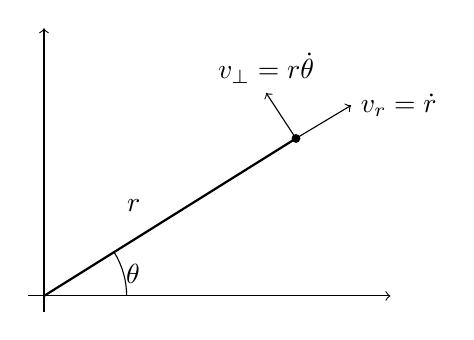
\begin{tikzpicture}
\draw[->] (-0.2,0) -- (4.4,0);
\draw[->] (0,-0.2) -- (0,3.4);
\draw[thick] (0,0) -- (3.2,2.0);
\fill (3.2,2.0) circle (1.6pt);
\draw (1.35,0.95) node[above left] {$r$};
\draw (1.05,0) arc (0:32:1.05);
\draw (0.92,0.28) node[right] {$\theta$};
\draw[->] (3.2,2.0) -- (3.9,2.42) node[right] {$v_r=\dot r$};
\draw[->] (3.2,2.0) -- (2.82,2.58) node[above] {$v_\perp=r\dot\theta$};
\end{tikzpicture}
\caption{Polar-coordinate geometry reconstructed from the lecture's argument. The velocity has a radial component \(\dot r\) and a perpendicular component \(r\dot\theta\).}
\end{figure}

Now take a central potential,
\begin{equation}
U=U(r),
\end{equation}
so that
\begin{equation}
L=\frac12 m\left(\dot r^2+r^2\dot\theta^2\right)-U(r).
\end{equation}
The transcript becomes noisy in the radial equation, and the lecture's stable emphasis lies elsewhere. The important point is that \(L\) does not depend explicitly on \(\theta\). Therefore \(\theta\) is a cyclic coordinate, and
\begin{equation}
\frac{\partial L}{\partial \dot\theta}=mr^2\dot\theta
\end{equation}
is conserved:
\begin{equation}
\frac{d}{dt}\left(mr^2\dot\theta\right)=0.
\end{equation}
Hence
\begin{equation}
mr^2\dot\theta=\text{constant}.
\end{equation}
This is conservation of angular momentum. It immediately explains the ice-skater effect invoked in the lecture: when \(r\) decreases, \(\dot\theta\) must increase to compensate.

We have thus arrived at the lecture's closing pattern:
\[
\text{translation invariance}\ \longrightarrow\ \text{linear momentum conservation},
\qquad
\text{rotational invariance}\ \longrightarrow\ \text{angular momentum conservation}.
\]

\section{Summary}

The lecture opens with a grand claim and then earns it step by step. First come two modest mathematical tools: integration by parts and the arbitrary-function lemma. Then comes the variational derivation:
\begin{equation}
\frac{d}{dt}\left(\frac{\partial L}{\partial \dot q_i}\right)=\frac{\partial L}{\partial q_i}.
\end{equation}
This equation is the bridge between a global least-action principle and a local differential law.

Only after that bridge is built does the lecture attach physical names to the objects in it. The derivative of the Lagrangian with respect to velocity becomes momentum; the derivative with respect to coordinate becomes generalized force; and the equation begins to read like \(F=ma\).

The examples then make the structure concrete. For one particle, the Euler--Lagrange equation reproduces Newton's law. For two interacting particles on a line, translation invariance yields conservation of total momentum. For a central force in polar coordinates, rotational invariance yields conservation of angular momentum. The chapter ends where the lecture ends: not with a single formula in isolation, but with the recognition of a pattern. Symmetry and conservation law belong together, and the principle of least action is the language in which that unity becomes visible.